\documentclass{beamer}

\usepackage[T2A]{fontenc}
\usepackage[utf8]{inputenc}
\usepackage[english,russian]{babel}
\input{settings.tex}

\newcommand{\myqrframe}{
	\begin{frame}
		\centerline{Слайды доступны на Github:}
		\bigskip
		\centerline{\mygit}
		\bigskip
		\myqr
	\end{frame}
}

\subtitle{Современные методы управления роботами}
\author{Сергей Савин}
\date{2026}

\title{Сертификаты устойчивости}
\centering



\begin{document}
	\maketitle
	
	
	\begin{frame}{Содержание}
		\begin{itemize}
			\item Неподвижные точки нелинейных систем: 1D
			\item Локальная устойчивость неподвижной точки
			\item Локальный анализ через линеаризацию
			\item Критерий линеаризации в 1D
			\item Когда линеаризация обращается в ноль
			\item Экспоненциальная устойчивость
			\item Локальная и глобальная устойчивость
			\item Критерии Ляпунова для глобальной устойчивости
			\item Пример: глобальная асимптотическая устойчивость
			\item Локальные критерии устойчивости Ляпунова
			\item Критерий Ляпунова для локальной экспоненциальной устойчивости
			\item Пример: локальная экспоненциальная устойчивость
		\end{itemize}
		
	\end{frame}
	
	
	
	
	\begin{frame}{Неподвижные точки нелинейных систем: 1D}
		\begin{flushleft}
			Рассмотрим линейную скалярную систему
			\[
			\dot{x} = ax, \qquad a \neq 0.
			\]
			
			Неподвижная точка (или равновесие) удовлетворяет \(	\dot{x} = 0\). Линейная система имеет \textbf{единственную неподвижную точку} \(x^\star = 0\).
			
			%\vspace{0.3cm}
			\bigskip
			
			Для нелинейной системы
			\[
			\dot{x} = f(x),
			\]
			может существовать \textbf{несколько неподвижных точек}, определяемых из условия \(f(x^\star)=0\). 
			
			
			%\vspace{0.3cm}
			\bigskip
			
			
			Например, следующая система:
			\[
			\dot{x} = -x+x^3 = x(x-1)(x+1).
			\]
			имеет три неподвижные точки \(x^\star \in \{-1,\,0,\,1\}\).
			
			
		\end{flushleft}
	\end{frame}
	
	
	
	
	\begin{frame}{Локальная устойчивость неподвижной точки}
		\begin{flushleft}
			{\small
			Рассмотрим \(\dot{x}=f(x)\) и пусть \(x^\star\) — неподвижная точка: \(f(x^\star)=0\).
			
			\begin{block}{Локальная устойчивость по Ляпунову}
				Равновесие \(x^\star\) называется \textbf{локально устойчивым}, если для любого
				\(\varepsilon>0\) существует \(\delta>0\) такое, что
				\[
				|x(0)-x^\star|<\delta
				\quad\Longrightarrow\quad
				|x(t)-x^\star|<\varepsilon,
				\qquad \forall t\geq 0.
				\]
			\end{block}
			
			\vspace{0.2cm}
			
			\begin{block}{Локальная асимптотическая устойчивость}
				Равновесие \(x^\star\) называется \textbf{локально асимптотически устойчивым (АУ)}
				если:
				
				\begin{enumerate}
					\item \(x^\star\) локально устойчиво;
					\item существует окрестность \(x^\star\) такая, что
					\[
					x(0)\ \text{в этой окрестности}
					\quad\Longrightarrow\quad
					\lim_{t\to\infty}x(t)=x^\star.
					\]
				\end{enumerate}
			\end{block}
		
		}
			
		\end{flushleft}
	\end{frame}
	
	
	
	
	\begin{frame}{Локальный анализ через линеаризацию}
		\begin{flushleft}
			\begin{adjustwidth}{-0.5cm}{-0.5cm}
				
				Дано \(\dot{x}=f(x)\) с неподвижной точкой \(x^\star\). Введем малое возмущение:
				\[
				\xi = x-x^\star.
				\]
				
				Тогда \(x=x^\star+\xi\) и разложение Тейлора дает:
				\[
				f(x^\star+\xi)
				=
				f(x^\star)
				+
				\frac{df}{dx}(x^\star)\xi
				+
				\mathcal{O}(\xi^2).
				\]
				
				Поскольку \(f(x^\star)=0\) и \(\dot{\xi} = f(x^\star+\xi)\):
				%
				\begin{align*}
					\dot{\xi}
					=
					\frac{df}{dx}(x^\star)\xi
					+
					\mathcal{O}(\xi^2).
				\end{align*}
				%
				\vspace{-0.9em}
				\begin{block}{Локальное линейное приближение}
					Для достаточно малых возмущений \(\xi\), если \(\frac{df}{dx}(x^\star)\neq 0\), линейный член доминирует:
					\[
					\dot{\xi}
					\approx
					\frac{df}{dx}(x^\star)\xi
					\]
				\end{block}
				
				Локальное поведение \(\leftrightarrow\) производная \(f\) в точке равновесия.
				
			\end{adjustwidth}
		\end{flushleft}
	\end{frame}
	
	
	
	\begin{frame}{Критерий линеаризации в 1D}
		\begin{flushleft}
			\begin{adjustwidth}{-0.5cm}{-0.5cm}
				
				Дано \(\dot{x}=f(x)\) с неподвижной точкой \(x^\star\). Линеаризованная динамика имеет вид:
				\[
				\dot{\xi}=f'(x^\star)\xi.
				\]
				
				\begin{block}{Критерий локальной устойчивости в 1D}
					\[
					\begin{array}{rcl}
						f'(x^\star)<0
						&\Longrightarrow&
						x^\star\ \text{локально асимптотически устойчива},\\[0.2cm]
						f'(x^\star)>0
						&\Longrightarrow&
						x^\star\ \text{неустойчива},\\[0.2cm]
						f'(x^\star)=0
						&\Longrightarrow&
						\text{линеаризация не дает ответа.}
					\end{array}
					\]
				\end{block}
				
				%\vspace{0.3cm}
				
				Для линейной системы
				\[
				\dot{x}=ax,
				\]
				имеем \(f(x)=ax\) и \(f'(x)=a\). Таким образом, известное условие линейной устойчивости
				\[
				a<0
				\]
				в точности совпадает с условием, основанным на производной.
				
			\end{adjustwidth}
		\end{flushleft}
	\end{frame}
	
	
	
	
	\begin{frame}{Когда линеаризация обращается в ноль}
		\begin{flushleft}
			\begin{adjustwidth}{-0.7cm}{-0.7cm}
				
				Предположим, что \(f(x^\star)=0\) и \(f'(x^\star)=0\). Тогда необходимо исследовать члены более высокого порядка. Пусть \(k\geq 2\) — порядок первой ненулевой производной:
				\[
				f^{(1)}(x^\star)=\cdots=f^{(k-1)}(x^\star)=0,
				\qquad
				f^{(k)}(x^\star)\neq 0.
				\]
				
				Локально,
				\[
				\dot{\xi}
				\approx
				\frac{f^{(k)}(x^\star)}{k!}\xi^k.
				\]
				
				
				\begin{block}{Критерий локальной устойчивости в 1D}
					\vspace{-0.9em}
					\[\begin{array}{rcl}
						\text{\(k\) четно}
						&\Longrightarrow&
						x^\star\ \text{неустойчива},\\[0.2cm]
						f^{(k)}(x^\star)>0
						&\Longrightarrow&
						x^\star\ \text{неустойчива},\\[0.2cm]
						\text{\(k\) нечетно и } f^{(k)}(x^\star)< 0 
						&\Longrightarrow&
						\text{\small локально асимптотически устойчива.}
					\end{array}
					\]
				\end{block}
				
				Применяя это к \(\dot{x}=-x^3\), получаем, что она асимптотически устойчива.
				
			\end{adjustwidth}
		\end{flushleft}
	\end{frame}
	
	
	
	
	\begin{frame}{Пример: \(\dot x = -x^3\), часть 1}
		\begin{flushleft}
			
			\begin{figure}
				\centering
				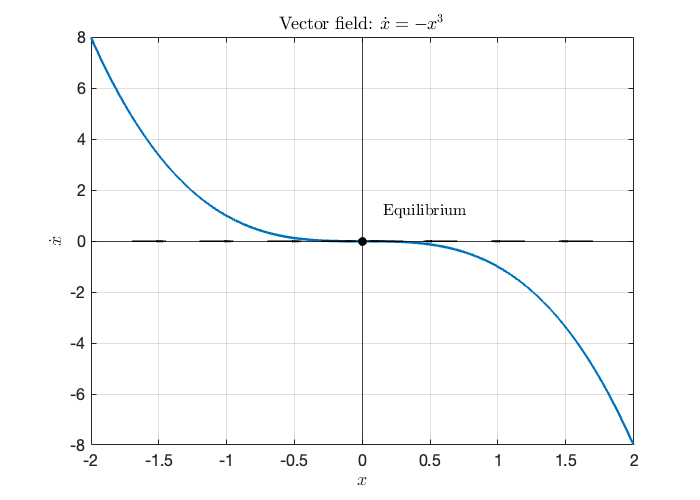
\includegraphics[width=0.95\linewidth]{example1}
				\caption{График функции \(\dot x = -x^3\)}
				\label{fig:example1}
			\end{figure}
			
			
		\end{flushleft}
	\end{frame}
	
	
	\begin{frame}{Пример: \(\dot x = -x^3\), часть 2}
		\begin{flushleft}
			
			\begin{figure}
				\centering
				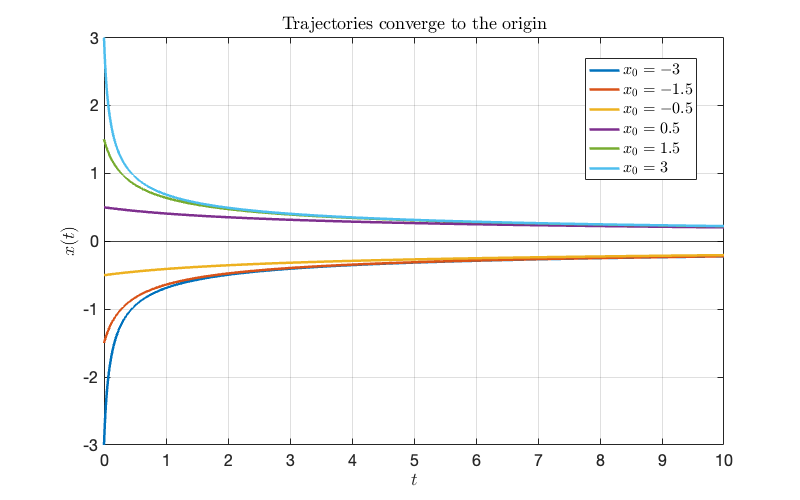
\includegraphics[width=1.0\linewidth]{example2}
				\caption{Решения ОДУ \(\dot x = -x^3\) при различных начальных условиях (см. приложение)}
				\label{fig:example1}
			\end{figure}
			
			
		\end{flushleft}
	\end{frame}
	
	
	
	
	\begin{frame}{Экспоненциальная устойчивость, 1}
		\begin{flushleft}
			Асимптотическая устойчивость требует только \(x(t)\to x^\star\) при \(t\to\infty\). Более сильным свойством является экспоненциальная устойчивость.
			
			\begin{block}{Локальная экспоненциальная устойчивость}
				Равновесие \(x^\star\) называется \textbf{локально экспоненциально устойчивым (ЭУ)}
				если существуют константы
				\[
				c>0,\qquad \lambda>0,\qquad \delta>0
				\]
				такие, что
				\[
				|x(0)-x^\star|<\delta
				\]
				влечет
				\[
				\boxed{
					|x(t)-x^\star|
					\leq
					c e^{-\lambda t}|x(0)-x^\star|,
					\qquad \forall t\geq 0.
				}
				\]
			\end{block}
			
			
		\end{flushleft}
	\end{frame}
	
	
	
	
	\begin{frame}{Экспоненциальная устойчивость, 2}
		\begin{flushleft}
			
			Для линейной стационарной системы \(\dot{x}=Ax\) асимптотическая устойчивость влечет экспоненциальную устойчивость:
			
			\[
			\boxed{\text{АУ} \iff \text{ЭУ}.}
			\]
			
			Для нелинейных систем, однако,
			\[
			\boxed{\text{ЭУ} \Longrightarrow \text{АУ},
				\qquad
				\text{но АУ} \centernot\Longrightarrow \text{ЭУ}.}
			\]
			
			Система
			\[
			\dot{x}=-x^3 
			\quad \text{с решением:} \quad
			x(t)
			=
			\frac{x(0)}
			{\sqrt{1+2x(0)^2t}},
			\]
			является примером: она асимптотически устойчива, но ее затухание
			\[
			|x(t)|\sim t^{-1/2}
			\]
			является полиномиальным, а не экспоненциальным.
			
		\end{flushleft}
	\end{frame}
	
	
	
	\begin{frame}{Локальная и глобальная устойчивость}
		\begin{flushleft}
			
			Различие между \textbf{локальной} и \textbf{глобальной} устойчивостью касается
			множества начальных условий, для которых выполняется свойство устойчивости.
			
			\begin{block}{Локальное vs. глобальное}
				Равновесие \(x^\star\) обладает данным свойством устойчивости \textbf{локально},
				если существует окрестность \(\mathcal{N}\) точки \(x^\star\) такая, что
				свойство выполняется для всех \(x(0)\in\mathcal{N}\).
				
				Оно обладает свойством \textbf{глобально}, если оно выполняется для всех
				\(x(0)\in\mathbb{R}^n\).
			\end{block}
			
			Примеры:
			\[
			\dot{x}=-x,\qquad \dot{x}=-x^3
			\]
			глобально асимптотически устойчивы, тогда как
			\[
			\dot{x}=-x+x^3
			\]
			локально асимптотически устойчива в \(x^\star=0\).
			
		\end{flushleft}
	\end{frame}
	
	
	
	\begin{frame}{Пример: \(\dot x = -x+x^3\), часть 1}
		\begin{flushleft}
			
			\begin{figure}
				\centering
				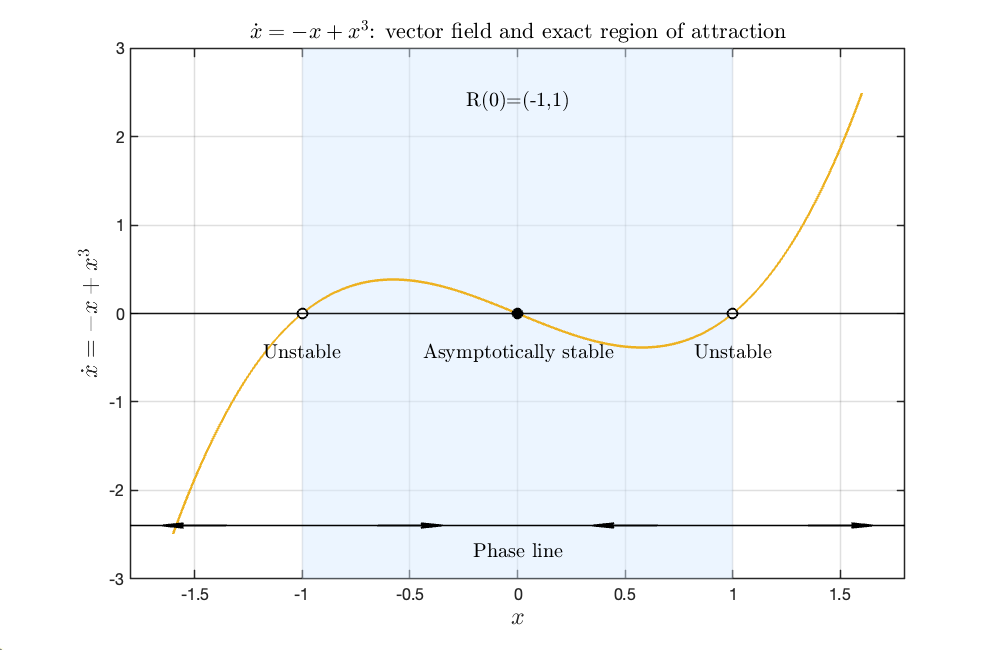
\includegraphics[width=1.0\linewidth]{example4}
				\caption{График функции \(\dot x = -x+x^3\)}
				\label{fig:example1}
			\end{figure}
			
			
		\end{flushleft}
	\end{frame}
	
	
	\begin{frame}{Пример: \(\dot x = -x+x^3\), часть 2}
		\begin{flushleft}
			
			\begin{figure}
				\centering
				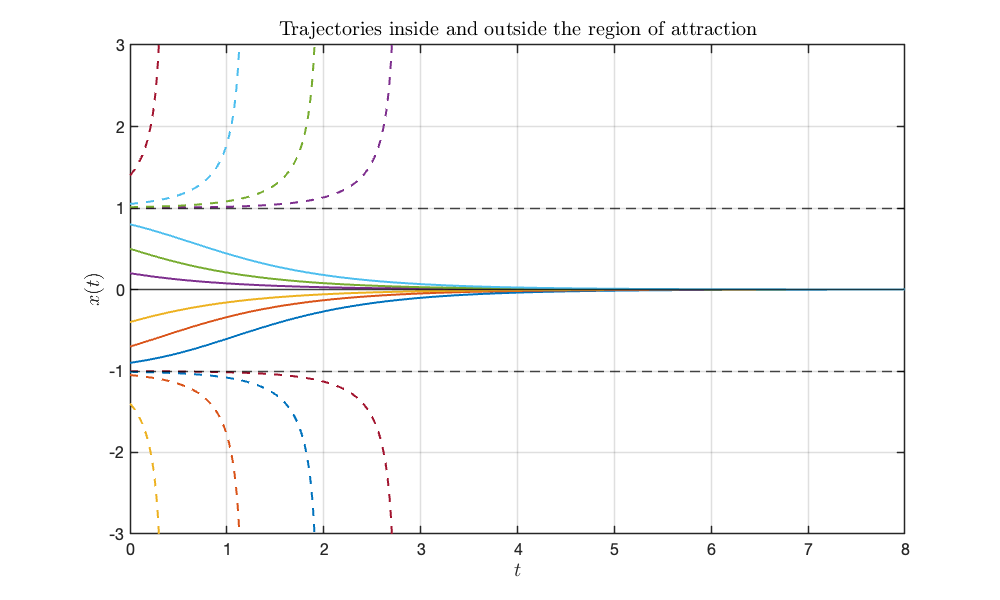
\includegraphics[width=1.05\linewidth]{example3}
				\caption{Решения ОДУ \(\dot x = -x+x^3\) при различных начальных условиях}
				\label{fig:example1}
			\end{figure}
			
			
		\end{flushleft}
	\end{frame}
	
	
	
	\begin{frame}{Критерии Ляпунова для глобальной устойчивости}
		\begin{flushleft}
			
			Рассмотрим
			\[
			\dot{x}=f(x), \qquad f(0)=0,
			\]
			и предположим, что существует непрерывно дифференцируемая функция
			\(V:\mathbb{R}^n\rightarrow\mathbb{R}\) такая, что
			\[
			V(0)=0, \qquad V(x)>0 \quad \forall x\neq 0,
			\]
			и \(V\) \textbf{радиально неограничена}:
			\[
			\|x\|\rightarrow\infty
			\quad\Longrightarrow\quad
			V(x)\rightarrow\infty.
			\]
			
			\hspace*{-0.5cm}
			\begin{minipage}{1.1\textwidth} 
				\begin{block}{Глобальные критерии Ляпунова}
					\[
					\dot V(x)\leq 0
					\quad\Longrightarrow\quad
					x^\star=0\ \text{глобально устойчива},
					\]
					\[
					\dot V(x)<0,\quad \forall x\neq0
					\quad\Longrightarrow\quad
					x^\star=0\ \text{\small глобально асимптотически устойчива.}
					\]
				\end{block}
			\end{minipage}
			
			
		\end{flushleft}
	\end{frame}
	
	
	
	\begin{frame}{Пример: глобальная асимптотическая устойчивость}
		\begin{flushleft}
			
			Рассмотрим
			\[
			\dot{x}=-x^3,
			\qquad x^\star=0.
			\]
			
			Выберем функцию Ляпунова
			\[
			V(x)=\frac{1}{2}x^2.
			\]
			
			Очевидно, \(V(x)>0\) для всех \(x\neq0\), и \(V(x)\rightarrow\infty\) при \(|x|\rightarrow\infty\).
			
			Ее производная вдоль траекторий равна
			\[
			\dot V(x)
			=
			x\dot{x}
			=
			-x^4<0,
			\qquad x\neq0.
			\]
			
			\[
			\boxed{\text{Итак, } x^\star=0\ \text{глобально асимптотически устойчива}.}
			\]
			
		\end{flushleft}
	\end{frame}
	
	
	
	
	\begin{frame}{Локальные критерии устойчивости Ляпунова}
		\begin{flushleft}
			Рассмотрим \(\dot{x}=f(x)\), с \(f(0)=0\). Предположим, что существует непрерывно дифференцируемая функция \(V(x)\)
			и окрестность \(\mathcal{N}\) точки \(0\) такие, что
			\[
			V(0)=0,
			\qquad
			V(x)>0 \quad \forall x\in\mathcal{N}\setminus\{0\}.
			\]
			
			\hspace*{-0.5cm}
			\begin{minipage}{1.1\textwidth} 
				\begin{block}{Локальные критерии Ляпунова}
					\[
					\dot V(x)\leq0
					\quad \forall x\in\mathcal{N}
					\quad\Longrightarrow\quad
					x^\star=0\ \text{локально устойчива},
					\]
					\[
					\dot V(x)<0
					\quad \forall x\in\mathcal{N}\setminus\{0\}
					\quad\Longrightarrow\quad
					x^\star=0\ \text{локально ас-ки устойчива}
					\]
				\end{block}
			\end{minipage}
			
		\end{flushleft}
	\end{frame}
	
	
	
	\begin{frame}{Критерий Ляпунова для локальной экспоненциальной устойчивости}
		\begin{flushleft}
			Рассмотрим \(\dot{x}=f(x)\), с \(f(0)=0\). Предположим, что в некоторой окрестности \(\mathcal{N}\) точки \(0\) существуют
			константы
			\[
			c_1>0,\qquad c_2>0,\qquad c_3>0
			\]
			такие, что
			\[
			c_1\|x\|^2
			\leq
			V(x)
			\leq
			c_2\|x\|^2,
			\]
			и
			\[
			\dot V(x)
			\leq
			-c_3\|x\|^2.
			\]
			
			\begin{block}{Критерий Ляпунова}
				Если эти неравенства выполняются локально, то \(x^\star=0\) является
				\textbf{локально экспоненциально устойчивой}.
			\end{block}
			
		\end{flushleft}
	\end{frame}
	
	
	
	
	\begin{frame}{Пример: локальная экспоненциальная устойчивость}
		\begin{flushleft}
			Рассмотрим
			\[
			\dot{x}=-x+x^3,
			\qquad x^\star=0.
			\]
			
			Выберем
			\[
			V(x)=\frac{1}{2}x^2.
			\]
			Тогда
			\[
			\dot V(x)
			=
			x \dot x
			=
			x(-x+x^3)
			=
			-x^2+x^4
			=
			-(1-x^2)x^2.
			\]
			
			Для \(|x|<\frac{1}{\sqrt{2}}\),
			\[
			\dot V(x)\leq-\frac{1}{2}x^2=-V(x).
			\]
			
			\[
			\boxed{x^\star=0\ \text{локально экспоненциально устойчива}.}
			\]
			
			Но обратите внимание: истинная область притяжения — не \(|x|<\frac{1}{\sqrt{2}}\), а \(|x|<1\).
			
		\end{flushleft}
	\end{frame}
	
	
	
	
	
	
	
	\begin{frame}{Литература}
		
		\begin{itemize}
			
			\item Kostas Margellos -- Nonlinear Systems (University of Oxford): \bref{https://kostasmargellos.github.io/assets/downloads/notes/C21_NonlinearSystems_LectureNotes.pdf}
			{C21 Nonlinear Systems}
			
			
			\item MIT OpenCourseWare -- Dynamics of Nonlinear Systems: \bref{https://ocw.mit.edu/courses/6-243j-dynamics-of-nonlinear-systems-fall-2003/resources/lec8_6243_2003/}
			{Lecture 8: Local Behavior at Eqilibria.}
			
			
			
		\end{itemize}
		
	\end{frame}
	
	
	
	\myqrframe
	
	
	
	\begin{frame}
		
		{\Large Приложение}
		
	\end{frame}
	
	
	\begin{frame}{Решения \(\dot{x}=-x^3\)}
		\begin{flushleft}
			
			Решения \(\dot{x}=-x^3\), где \(x(0) = x_0 > 0\), имеют вид:
			\[
			x(t)
			=
			\frac{x_0}
			{\sqrt{1+2 x_0^2t}} 
			= 
			\frac{1}
			{\sqrt{\frac{1}{x_0^2}+2t}} 
			\]
			
			При \(t \gg \frac{1}{x_0^2}\) решение близко к \(\frac{1}{\sqrt{2t}}\):
			\[
			x(t)
			\sim
			\frac{1}{\sqrt{2t}}, \quad t \gg \frac{1}{x_0^2}.
			\]
			
			Таким образом, любое решение приближается к \(h(t) = \frac{1}{\sqrt{2t}}\) при достаточно больших \(t\).
			
		\end{flushleft}
	\end{frame}



\end{document}
